\documentclass[__main__.tex]{subfiles}
\begin{document}
	
	\qtitle{Ч}{10}
	Эксперимент Штерна-Герлаха. Гипотеза спина электрона. Оператор проекции спина на выделенное направление. Эксперименты с поляризованным пучком электронов.\\ 
	
	\textbf{Эксперимент Штерна-Герлаха}\\
	На атом обладающий магнитным моментом $\vec{\mu}$, в неоднородном магнитном поле $\vec{B}$ должна действовать сила
	\begin{gather*}
		\vec{f} = \left(\vec{\mu}\cdot\nabla\right)\vec{B}
	\end{gather*}
	Чтоб рассуждать было проще, пусть $B_x, B_y = 0$  и $B_z \neq 0$, тогда
	\begin{gather*}
		\vec{f} = \left(\mu_x\partial_xB_z+\mu_y\partial_yB_z+\mu_z\partial_zB_z\right)\vec{e}_z
	\end{gather*}
	направлена либо по либо против $z$. Пусть неоднородность создана лишь вдоль $z$ тогда $\partial_xB_z=0; \partial_yB_z=0$\\\\
	Опыт выглядит довольно просто: направим пучок атомов в область неоднородного магнитного поля и посмотрим что будет на выходе из этой области.
	%probably will be useful to put image
	В области неоднородного магнитного поля на атомы с $\mu_z \neq 0$ действует сила $f_z \sim \mu_z$; в результате они отклоняются от первоначального направления; величина отклонения тем больше, чем больше $|\mu_z|$; вверх или вниз зависит от знака $\mu_z$.
	Согласно квантовой механике $\mu_z$ квантуется $\Rightarrow$ исходный пучок обязан расщепиться на число пучков, равное числу разрешенных $\mu_z$. В итоге должно получится что-то вроде(\textbf{пространственное квантование} -- набор эквидистантных пятен на экране):
	\begin{figure}[h]
		\center{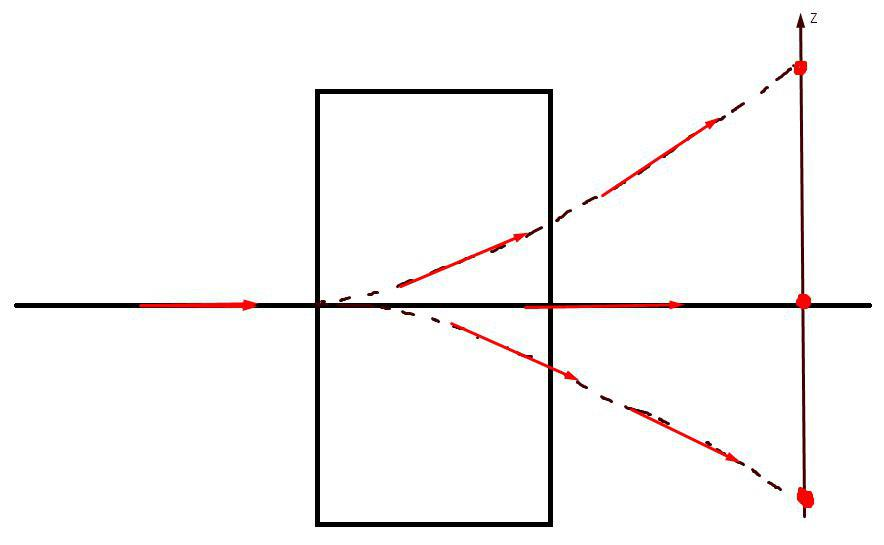
\includegraphics[width=0.9\linewidth]{ch-18}}
	\end{figure}

	\textbf{Гипотеза спина электрона}\\
	Подсчитаем число пучков на выходе из неоднородного $\vec{B}$. Вопрос: Сколько возможных $\mu_z$ ?
	\begin{gather*}
		\mu_z = -\mu_Bm
	\end{gather*}
	где $\mu_B$ - магнетон Бора.\\
	При фиксированном $l$ число возможных $m$ составляет $2l+1$ и учитывая, что $l,n \in N$, приходим к выводу, что число возможных $m$ - нечетное. Проверим это:\\
	Для этого пропустим пучок атомов водорода с $l=0$ через область неоднородного магнитного поля. Поскольку $l = 0 \Rightarrow m = 0 \Rightarrow \mu_z = 0 \Rightarrow$ пучок должен проследовать прямо в центр экрана, НО это не так - он расщепляется на две составляющие! Таким образом приходиться предположить, что электрон обладает собственным моментом импульса или спином, которому соответствует некоторый магнитный момент. Приходим к определению полного момента импульса частицы:
	\begin{gather*}
		\hat{J} = \hat{L}+\hat{S}
	\end{gather*} 
	где $\hat{L}$ - орбитальный момент, $\hat{S}$ - спин.\\\\
	Ввиду того (как оказалось), что электрон обладает внутренней степенью свободы(спином), то теперь для того, чтобы охарактеризовать его стационарные состояния в поле ядра нам потребуется уже не 3 квантовых числа а четыре (добавляется спиновое квантовое число - $m_s$)\\\\
	
	\textbf{Оператор проекции спина на выделенное направление.}\\
	Пусть $\vec{n} = (n_x,n_y,n_z)$ есть единичный вектор, указывающий направление ($n^2_x+n^2_y+n^2_z = 1$), тогда оператор $\hat{S}\vec{n} = \hat{S}_xn_x+\hat{S}_yn_y+\hat{S}_zn_z$ называется оператором проекции спина на направление $\vec{n}$. Его можно представить в виде:
	\begin{gather*}
		\left(\hat{S}\vec{n}\right) = \frac{\hbar}{2}\left(\hat{\sigma}\vec{n}\right)=\frac\hbar2\left(\hat{\sigma}_xn_x+\hat{\sigma}_yn_y+\hat{\sigma}_zn_z\right) = \frac{\hbar}{2}\begin{pmatrix}
			n_z & n_x-in_y\\
			n_x+in_y & -n_z
		\end{pmatrix}
	\end{gather*}
	\textbf{Эксперименты с поляризованным пучком электронов}\\\\
	Давайте получим электрон в состоянии <<спин - вверх>>. Словосочетание <<спин - вверх>> -- удобное сокращение фразы: состояние в котором проекция спина на выделенное направление положительна. Для того, чтобы  получить электрон в состоянии <<спин - вверх>>, берем прибор Штерна-Герлаха и ориентируем его в пространстве так, чтобы градиент магнитного поля был по $Z$; затем пропускаем через область неоднородного магнитного поля пучок электронов и ставим <<заглушку>> в месте, откуда выходят электроны в состоянии <<спин-вниз>>. В результате останутся электроны с положительно ориентированной по $Z$ проекцией спина - в итоге получим поляризованный пучок.  
\end{document}